\section{Cameras}

In graphics, a camera projects a 3D scene onto a 2D plane which
can be displayed on a screen. If we model the camera as a point,
then the problem becomes a linear algebra issue of projecting a
set of points onto a plane determined by the camera. We must
display only surfaces not obscured by other surfaces, not accounting
for things like transparency.

\begin{figure}
    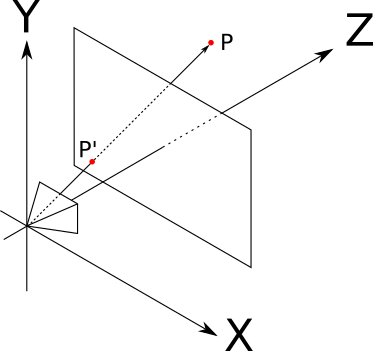
\includegraphics{images/camera.png}
    \caption{Camera}
    \label{fig:camera}
\end{figure}

A \emph{pose} consists of three translations and three rotations.
Setting each results in a unique camera pose in 3D space.

\marginnote{There are several ways to approximate the way the human
    eye sees, the method used in this class is called the planar pinhole method.
    There are many, many other camera models, for instance thin lens camera,
    orthographic camera, spherical camera, fisheye camera.}